\begin{landscape}
\begin{figure}[ht!]
  \centering
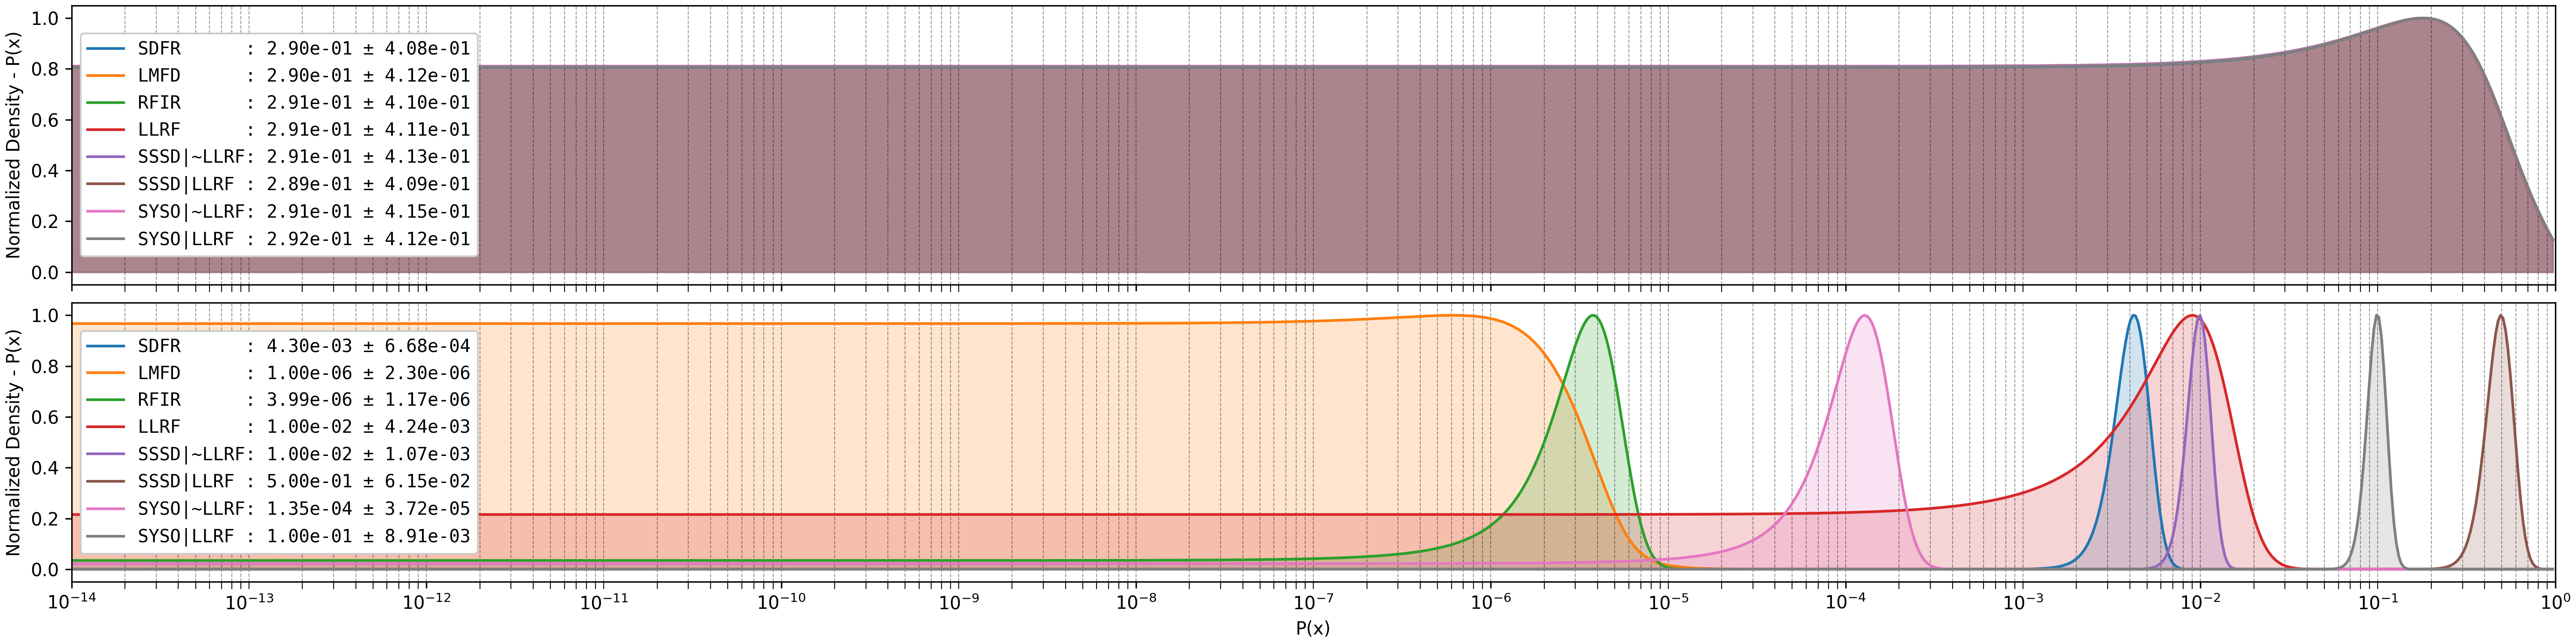
\includegraphics[width=\textwidth]{parts/4_learning/1_param/figs/conditional_events_prior.png}
    \caption{Initial vs Target Functional Event Probability Distributions}
    \label{fig:conditionals_initial}
\end{figure}

\begin{figure}[hb!]
\centering
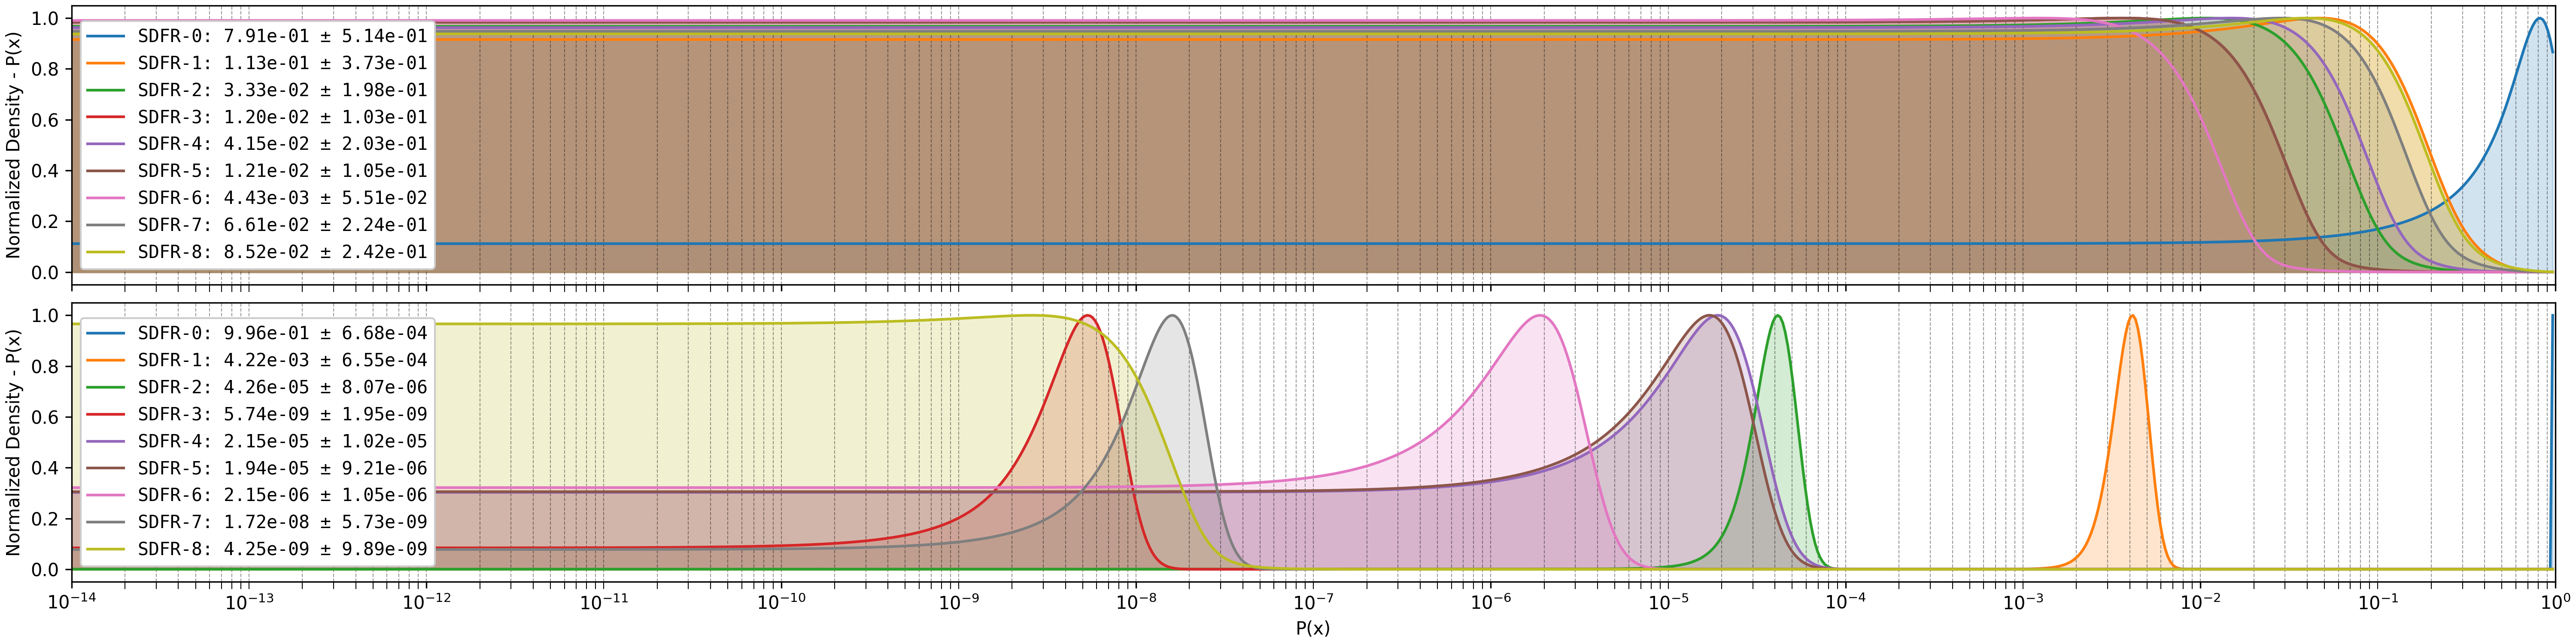
\includegraphics[width=\textwidth]{parts/4_learning/1_param/figs/end_states_prior.png}
    \caption{Initial vs Target End-State Frequency Distributions}
     \label{fig:end-states_initial}
\end{figure}
\end{landscape}

\clearpage
\begin{landscape}
\begin{table}[ht!]
\centering
\caption{Estimated vs Target Functional Event Probabilities Summarized}
\label{tab:conditional_estimated}
\scriptsize
\sisetup{table-format=1.2e-2}
\begin{tabular}{
    l
    S[table-format=1.2e-2]
    S[table-format=1.2e-2]
    S[table-format=1.2e-2]
    S[table-format=1.2e-2]
    S[table-format=1.2e-2]
    S[table-format=1.2e-2]
    S[table-format=1.2e-2]
    S[table-format=1.2e-2]
    S[table-format=1.2e-2]
    }
\toprule
\multirow{2}{*}{Event} & \multicolumn{3}{c}{$5^{th}$ Percentile} & \multicolumn{3}{c}{Mean} & \multicolumn{3}{c}{$95^{th}$ Percentile} \\
\cmidrule(lr){2-4} \cmidrule(lr){5-7} \cmidrule(lr){8-10}
& {Estimated} & {Target} & {Error\footnotemark} & {Estimated} & {Target} & {Error\footnotemark[\value{footnote}]} & {Estimated} & {Target} & {Error\footnotemark[\value{footnote}]} \\
\midrule
SDFR & 3.28e-03 & 3.30e-03 & -2.30e-05 & 4.24e-03 & 4.30e-03 & -5.97e-05 & 5.37e-03 & 5.47e-03 & -1.07e-04 \\
LMFD & 4.39e-08 & 4.29e-08 & 9.85e-10  & 1.00e-06 & 9.99e-07 & 7.13e-10  & 3.70e-06 & 3.70e-06 & -5.09e-09 \\
RFIR & 2.49e-06 & 2.39e-06 & 9.28e-08  & 4.13e-06 & 4.00e-06 & 1.29e-07  & 6.32e-06 & 6.15e-06 & 1.71e-07  \\
LLRF & 4.73e-03 & 4.72e-03 & 1.94e-05  & 9.93e-03 & 9.99e-03 & -6.36e-05 & 1.77e-02 & 1.79e-02 & -2.25e-04 \\
$\text{SSSD} \mid \overline{\text{LLRF}} $\footnotemark[2] & 8.72e-03 & 8.35e-03 & 3.68e-04  & 1.01e-02 & 1.00e-02 & 5.37e-05  & 1.15e-02 & 1.19e-02 & -3.31e-04 \\
$\text{SSSD} \mid \text{LLRF} $ & 4.93e-01 & 4.06e-01 & 8.74e-02  & 4.94e-01 & 5.00e-01 & -5.48e-03 & 4.96e-01 & 6.07e-01 & -1.11e-01 \\
$\text{SYSO} \mid \overline{\text{LLRF}} $ & 8.24e-05 & 8.33e-05 & -9.54e-07 & 1.36e-04 & 1.35e-04 & 8.31e-07  & 2.07e-04 & 2.03e-04 & 3.85e-06  \\
$\text{SYSO} \mid \text{LLRF} $ & 8.54e-02 & 8.60e-02 & -6.49e-04 & 9.89e-02 & 1.00e-01 & -1.11e-03 & 1.14e-01 & 1.15e-01 & -1.66e-03 \\
\bottomrule
\end{tabular}
\end{table}

\begin{figure}[hb!]
  \centering
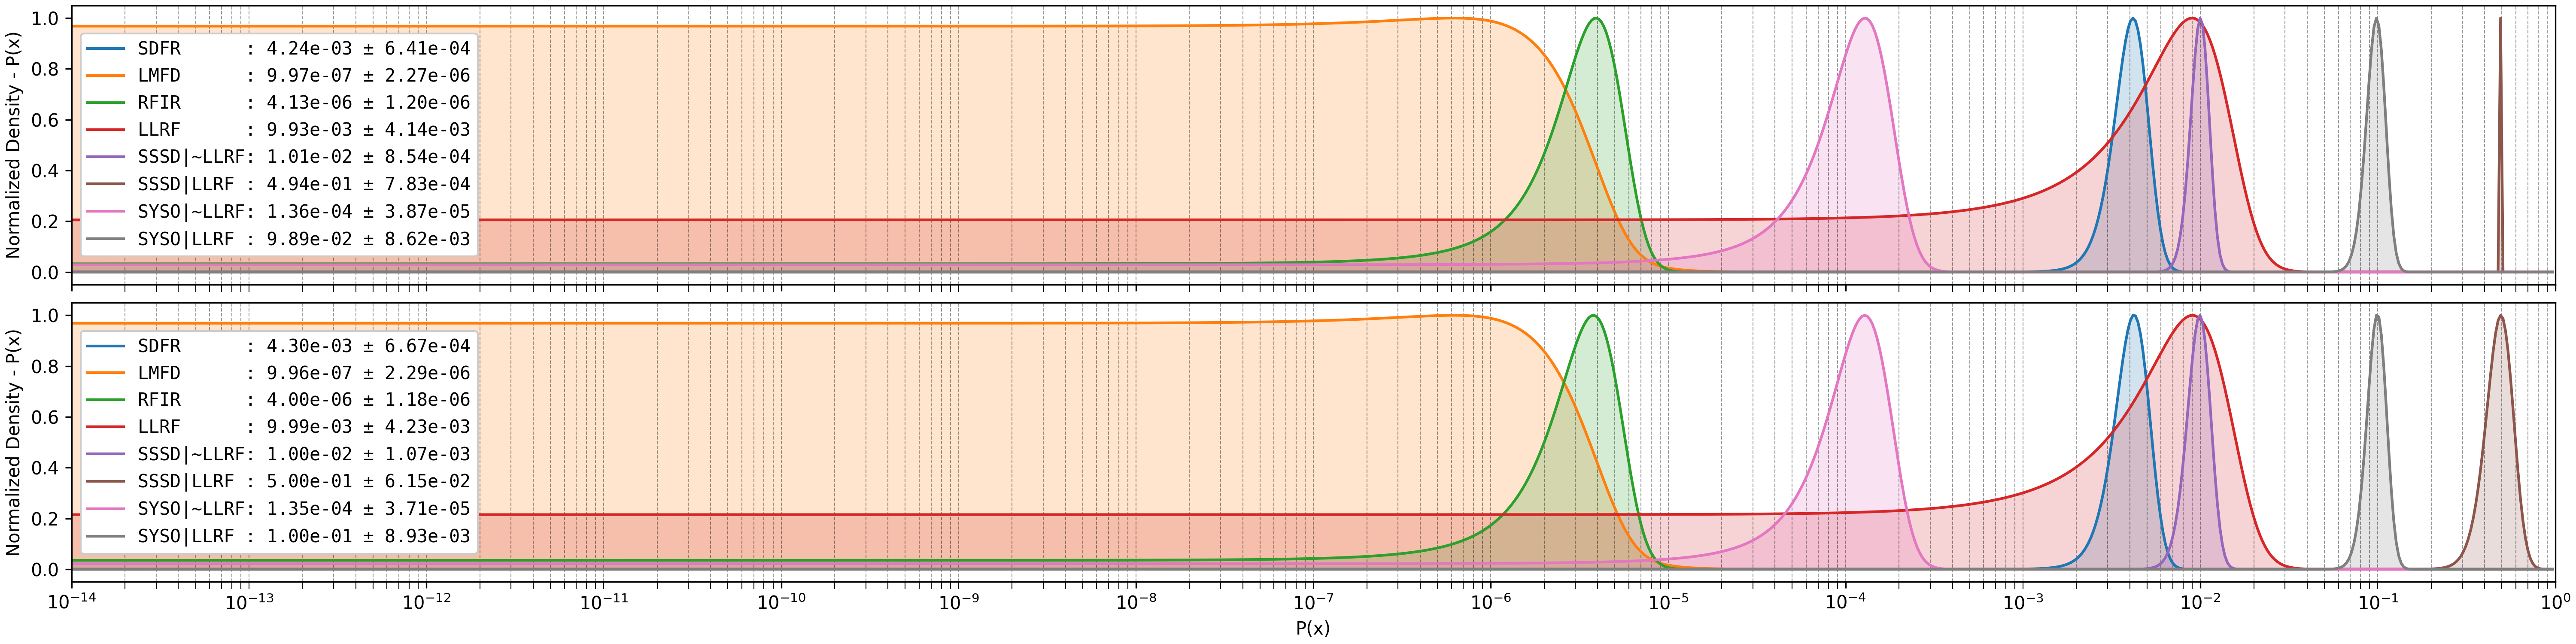
\includegraphics[width=\textwidth]{parts/4_learning/1_param/figs/conditional_events_predicted.png}
    \caption{Estimated vs Target Functional Event Probability Distributions}
    \label{fig:conditional_estimated}
\end{figure}

\footnotetext[1]{[Estimated - Target], negative values represent underestimates.}
\footnotetext[2]{$ A \mid \overline{B} $: event A conditional on the non-occurrence of event B.}
\end{landscape}
\clearpage

\clearpage
\begin{landscape}

\begin{table}[ht!]
\centering
\caption{Estimated vs Target End-State Frequencies Summarized}
\label{tab:summary}
\scriptsize
\sisetup{table-format=1.2e-2}
\begin{tabular}{
    l
    S[table-format=1.2e-2]
    S[table-format=1.2e-2]
    S[table-format=1.2e-2]
    S[table-format=1.2e-2]
    S[table-format=1.2e-2]
    S[table-format=1.2e-2]
    S[table-format=1.2e-2]
    S[table-format=1.2e-2]
    S[table-format=1.2e-2]
    }
\toprule
\multirow{2}{*}{Event} & \multicolumn{3}{c}{$5^{th}$ Percentile} & \multicolumn{3}{c}{Mean} & \multicolumn{3}{c}{$95^{th}$ Percentile} \\
\cmidrule(lr){2-4} \cmidrule(lr){5-7} \cmidrule(lr){8-10}
& {Estimated} & {Target} & {Error\footnotemark[3]} & {Estimated} & {Target} & {Error\footnotemark[\value{footnote}]} & {Estimated} & {Target} & {Error\footnotemark[\value{footnote}]} \\
\midrule
SDFR-0\footnotemark[4] & 9.95e-01 & 9.95e-01 & 1.08e-04 & 9.96e-01 & 9.96e-01 & 5.98e-05 & 9.97e-01 & 9.97e-01 & 2.30e-05 \\
SDFR-1 & 3.21e-03 & 3.23e-03 & -2.26e-05 & 4.16e-03 & 4.22e-03 & -5.86e-05 & 5.27e-03 & 5.37e-03 & -1.06e-04 \\
SDFR-2 & 3.12e-05 & 3.07e-05 & 5.81e-07 & 4.22e-05 & 4.26e-05 & -3.56e-07 & 5.52e-05 & 5.69e-05 & -1.70e-06 \\
SDFR-3 & 3.15e-09 & 3.15e-09 & -7.36e-12 & 5.73e-09 & 5.74e-09 & -1.31e-11 & 9.33e-09 & 9.35e-09 & -2.39e-11 \\
SDFR-4 & 9.62e-06 & 9.22e-06 & 4.07e-07 & 2.13e-05 & 2.15e-05 & -1.90e-07 & 3.94e-05 & 4.07e-05 & -1.33e-06 \\
SDFR-5 & 8.47e-06 & 8.31e-06 & 1.66e-07 & 1.88e-05 & 1.94e-05 & -5.87e-07 & 3.47e-05 & 3.67e-05 & -2.04e-06 \\
SDFR-6 & 9.10e-07 & 9.07e-07 & 3.35e-09 & 2.06e-06 & 2.15e-06 & -9.10e-08 & 3.85e-06 & 4.13e-06 & -2.86e-07 \\
SDFR-7 & 9.84e-09 & 9.58e-09 & 2.64e-10 & 1.75e-08 & 1.72e-08 & 3.08e-10 & 2.82e-08 & 2.79e-08 & 3.17e-10 \\
SDFR-8 & 1.81e-10 & 1.80e-10 & 1.85e-12 & 4.18e-09 & 4.24e-09 & -5.50e-11 & 1.56e-08 & 1.58e-08 & -2.53e-10 \\
\bottomrule
\end{tabular}
\end{table}

\begin{figure}[ht!]
\centering
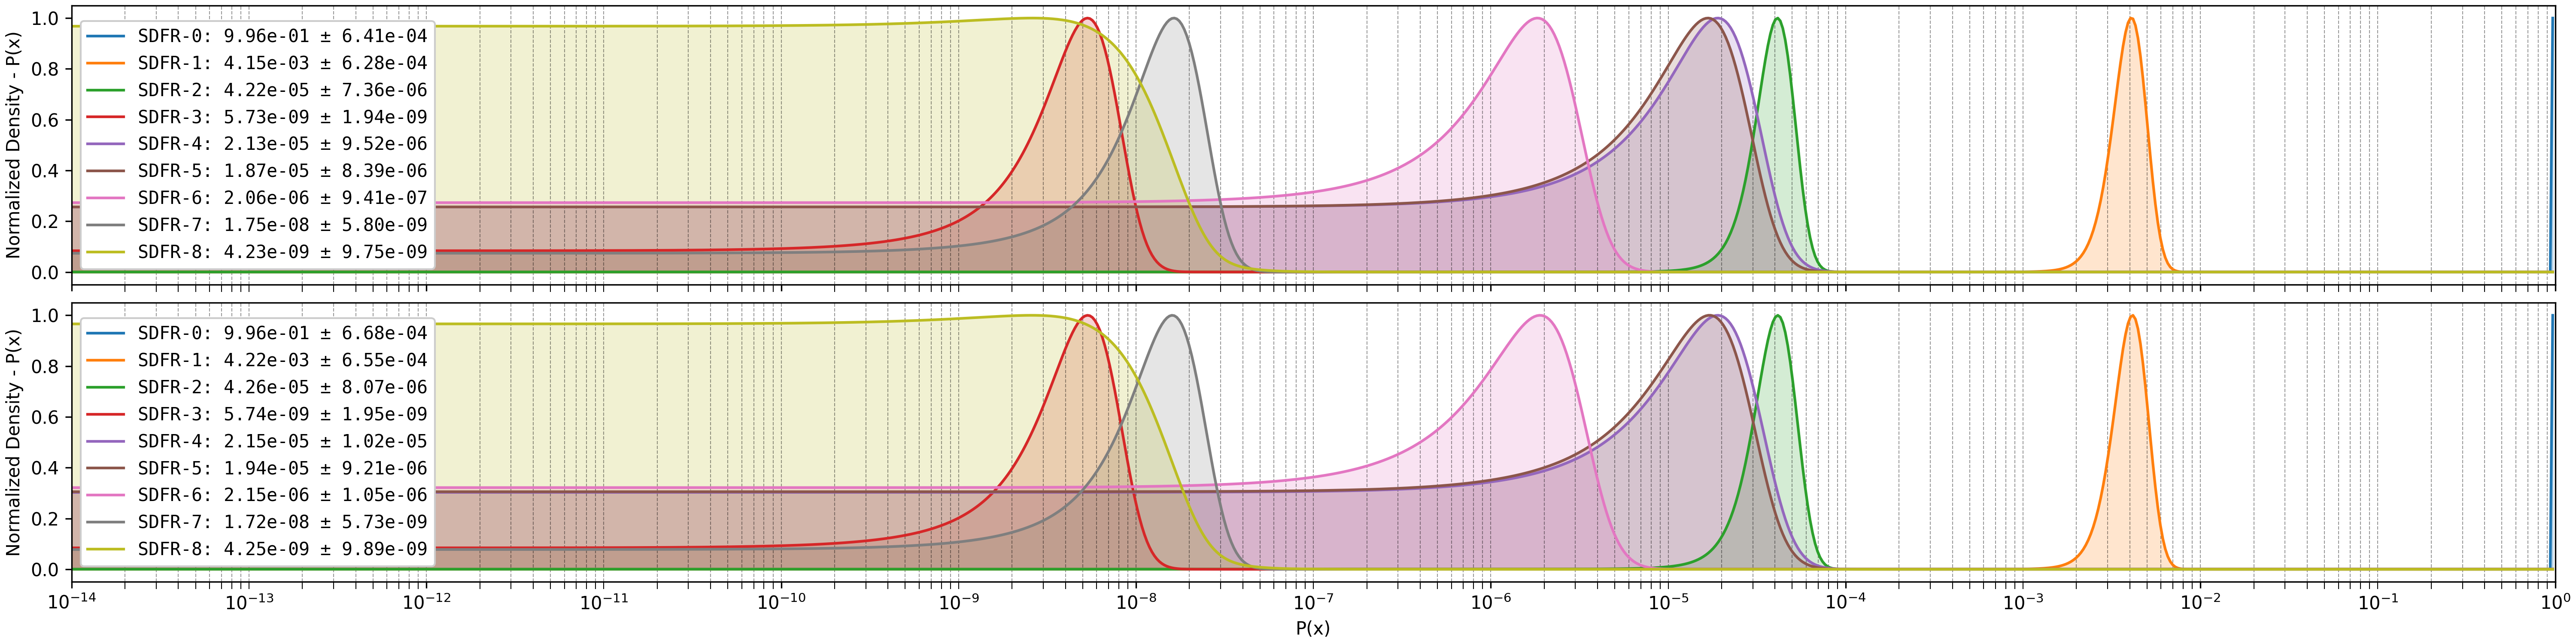
\includegraphics[width=\textwidth]{parts/4_learning/1_param/figs/end_states_predicted.png}
    \caption{Estimated vs Target End-State Frequency Distributions}
    \label{fig:end-states_estimated}
\end{figure}

\footnotetext[3]{[Estimated - Target], negative values represent underestimates.}
\footnotetext[4]{The likelihood of no SDFR. Computed by subtracting all end-state frequencies from the total probability.}
\end{landscape}
\clearpage